As the number of data points increases, it is difficult to perform meaningful analysis using the methods mentioned in earlier. In state model analysis, the sequential data is converted to nodes and edges of a graph which represents the entire data and states.  State model analysis is helpful when the number of data points are more and when there is a repetition of a set of data points. State model provides information about the probability of occurrence of each state and the transitional probability of each activity.  This information is helpful to use to statistically evaluate usage patters in a predictive way, to quantify the weighted profile of use cases for the system, and to identify misuse cases.

However, when the number of states are more, the WDG becomes more complex and hence difficult to understand. in such cases, identifying the most active states and edges provides information about the important activities in the data set. This approach is more suitable when the number of states in the data set is less than 30. If the number of states is more, either use some other analysis or combine the states to get more meaningful data. (for example, if the data set consists of the interactions of methods in a source code and the number of methods is quite high, it is better to do the analysis at the class level which provides more insight to the relationships.

Usage data can be analyzed with state models by transforming the serially ordered events in a sequence data to a Weighted Directed Graph (WDG) data structure. Only the information needed for the analysis need to be maintained and condensed into a compact view of the log file. We can abstract the information in the log line to any level, such as, event level, method level, class level, file level, sub-module level, or module level. In the sequence data, each event is important as a standalone event. However, in the WDG representation, the importance shifts to adjacent pairs of events. We do this type of a transformation to record the order in which events happened. Therefore, each unique event in the sequence data is represented by a unique node in the WDG. An edge exists from one node (head) to another (tail) if there is an occurrence of the event representing the tail node immediately after the event representing the head node in the original log file. For example if event B follows event A in the log file, then there is directed edge from node A to node B in the WDG. The edges are labeled with the number of times this transition has occurred.  For example if B occurs a fifty times after A in the log file, then the edge from node A to node B in the WDG is labeled with 50. Typically, we keep track of the actual count as the weight of the edge, when building the graph. In the graph we display the percentage value as the label. This percentage is proportional to the total number of transitions.  The cumulative probability of out-edges of a node is 1. The transitional probabilities of each out-edges are calculated by dividing the number of transactions of that out-edge with the sum of all outward transactions from that node. We could also store the dynamic parameter information in each log line as a list along the edges. 

As an example, consider a sample log file \ref{samplelogfile} and the corresponding TML file are given below. The TML script has information about the nodes, the out edges from each node along with the number of transitions from each node to another. This TML script is used in JUMBL to arrive at the state probabilities of each node. State probabilities give information about the percentage of usage of each node. Corresponding graph is depicted in Fig. \ref{op-profile-example}


\begin{figure}
\label{samplelogfile}
\hrulefill
\begin{verbatim}
2013-03-21 18:18:32Z,A
2013-03-21 18:18:33Z,B
2013-03-21 18:20:49Z,C
2013-03-21 18:20:50Z,A
2013-03-21 18:20:56Z,B
2013-03-21 18:20:57Z,A
2013-03-21 18:21:08Z,C
2013-03-21 18:21:08Z,D
2013-03-21 18:21:08Z,E
2013-03-21 18:21:08Z,A
\end{verbatim}
\hrulefill
\caption{Sample Log File to Convert to State Model}
\end{figure}

%the other example is aligned with the sample graph thus better.
%As an example of WDG, consider a simple log file where the activities are separated by commas. $1-2, 2-3, 3-4, 4-5, 5-4, 4-5, 5-4, 4-6, 6-7, 7-5, 5-4, 4-5, 5-4, 4-5, 5-8, 8-9$. The events in the log file are mapped to their corresponding event IDs: $1, 2, 3, 4, 5, 4, 5, 4, 6, 7, 5, 4, 5, 4, 5, 8, 9$. Each node is a unique event. An edge between nodes 1 and 2 signifies that the event 2  appears after event 1  in the log file. The labels on the edges have the actual count and could have the transitional probabilities as well. The transitional probability from node 1 to node 2 is 1.0, whereas the transitional probability from node 4 to node 6 is 0.2.  This is depicted in Fig \ref{op-profile-example}.
 
\begin{figure}[h]
  \centering
  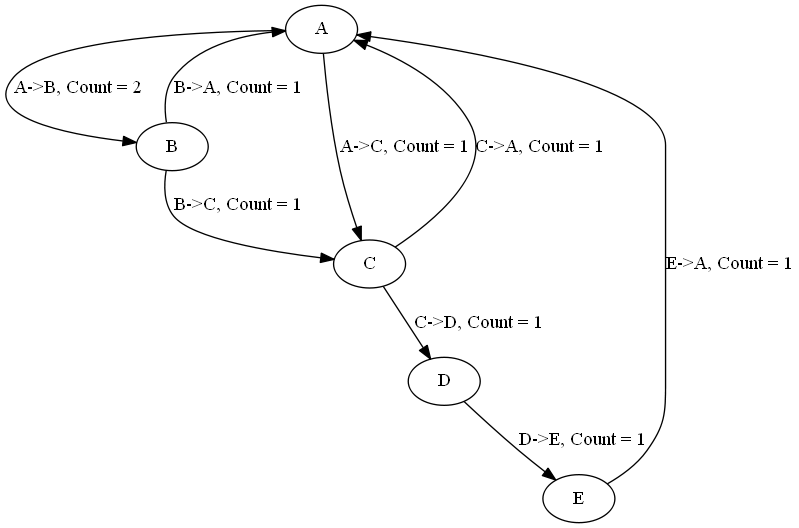
\includegraphics[scale=.40]{../Graphics/op-profile-example.png}
  \caption{Weighted Directed Graph of the Example Log}\label{op-profile-example}
\end{figure}

JUMBL (Java Usage Model Builder Library) developed by Software Quality Research Laboratory (SQRL) of University of Tennessee \cite{jumbl} can be used for developing operational profile and calculating the probability of usage by each state of the operational profile. JUMBL is a collection of tools to support automated, model-based, statistical testing of systems \cite{jug}. JUMBL helps in

\begin{itemize}
\item Constructing usage models from component states
\item Generating tests in various ways
\item Converting tests to executable data to support test automation, and
\item Assessing testing by providing test measures, including expected system reliability in the field.
\end{itemize}

A WDG along with the transitional probability are used to determine the state probabilities of each component . We have used JUMBL to create the state probabilities \cite{anil}. We have converted the WDG to JUMBL readable TML \cite{tug} language. 
%hmm, without these tools this no longer works as a how-to.  Can the tool code be provided?
We have developed tools, which will mine the log file and convert the log file to an adjacency matrix representation with the number of transitions from each node, which is translated directly to TML script. 

Using state models, a sequence data with hundreds of thousands of lines can be quickly converted to more meaningful graphical representation using this method. Once the TML file is generated, we can use JUMBL to find out the state probabilities of each states. Using the state probability and the usage patterns we can arrive conclusions and can visualize them easily as  shown in figure \ref{op-profile-example}.

%Trying this on without the following examples.  They don't really add much and raise more questions than they answer.  I hope reference take care of the how to in this case.


%
%\begin{figure}
%\label{sampleTML}
%\hrulefill
%\begin{verbatim}
%($ fill(1) $)
%model testlog
%//use this before each transition to show probability ($0.10$)
%
%source [A]
%($2$)"Count=2 (A->B), TimeElapsed= 7secs" [B]
%($1$)"Count=1 (A->C), TimeElapsed= 11secs" [C]
%
%[B]
%($1$)"Count=1 (B->C), TimeElapsed= 136secs" [C]
%($1$)"Count=1 (B->A), TimeElapsed= 1secs" [A]
%
%[C]
%($1$)"Count=1 (C->A), TimeElapsed= 1secs" [A]
%($1$)"Count=1 (C->D)" [D]
%
%[D]
%($1$)"Count=1 (D->E)" [E]
%
%[E]
%($1$)"Count=1 (E->A)" [A]
%
%
%"exit" [Exit]
%
%end 
%\end{verbatim}
%\hrulefill
%\caption{Sample TML for a State Model}
%\end{figure}



%%I commented these out because they were out in space in the document and not well supported by the text.  You probably cut the text because of other comments.  Anyhow does it make sense to stick with one WDG example based on the state model shown in text above?  Seems OK to me so far. 

%\begin{figure}
%  \centering
%  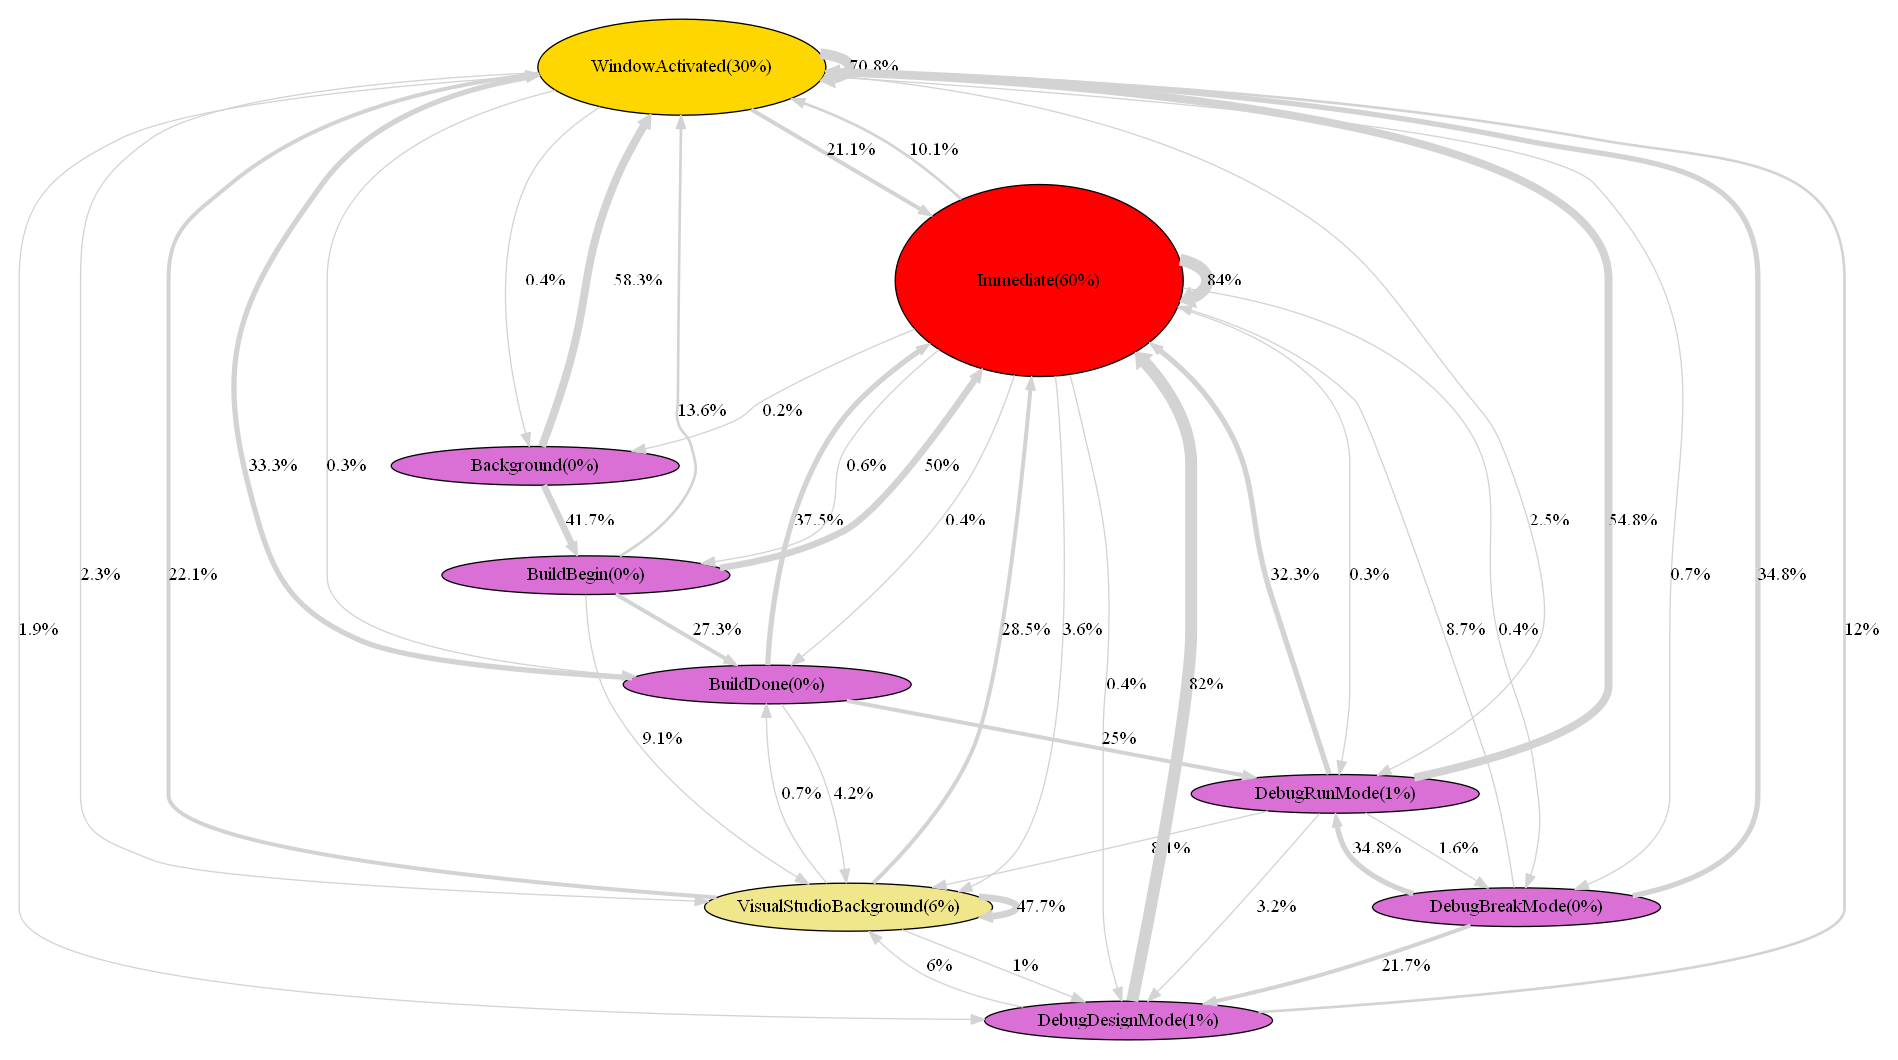
\includegraphics[scale=.15]{../Graphics/log_with_color.png}
%  \caption{WDG example with probability}\label{fig:log_with_color}
%\end{figure}

%\begin{figure}
%  \centering
%  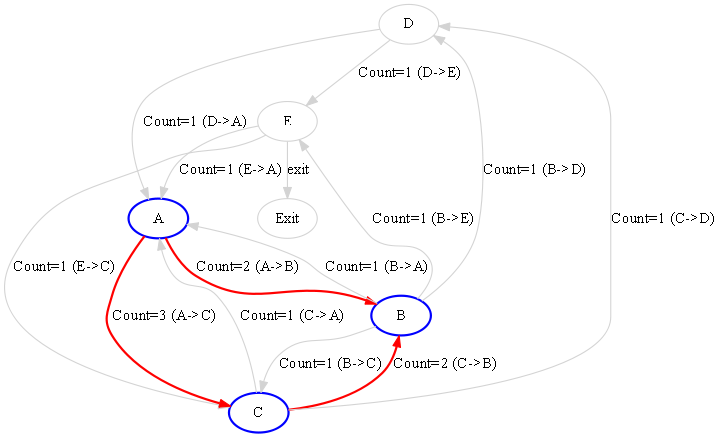
\includegraphics[scale=.50]{../Graphics/sample_log.png}
%  \caption{WDG example with count}\label{fig:sample_log}
%\end{figure}

 


